\documentclass[12pt]{article}
\usepackage[margin=1in]{geometry}
\usepackage{amsmath}
\usepackage{graphicx}
\usepackage{setspace}
\usepackage{subcaption}
\usepackage{listings}
\usepackage[italicdiff]{physics}
\usepackage{natbib}
\usepackage{epstopdf}
\lstset{breaklines=true, tabsize = 3}

\author{Jonathan Bunton}
\title{Solving for the Steady-State Solution \\ of the Heat Equation in a Cubic Satellite}
\date{\today}

\begin{document}
\maketitle
\onehalfspacing
\begin{abstract}
Before launching objects into low orbit space, it is prevalent to study their expected behavior in given conditions.  One particular behavior worth investigating is the eventual thermal characteristics of the system.  To do this, we can utilize the fact that in general, the temperature of a material over time $T(x,y,z,t)$ is governed by the heat equation. \cite{heateq} This partial differential equation is given by:
\begin{equation*}
\nabla^2T = \frac{1}{\alpha}\dv{T}{t}
\end{equation*}
In the eventual steady-state situation, the temperature $T(x,y,z,t)$ ceases to change with time.  Put mathematically, we seek a solution to:
\begin{equation*}
\nabla^2T = 0.
\end{equation*}
To even begin to solve this equation, we require proper boundary conditions. In this particular case, we consider a tidally locked 0.1 meter cubic mass of polystyrene foam, coated with polysilicon and containing a 0.4 meter cubic aluminum mass which stays at a constant 100 K.  This will serve as our ``satellite."  We assume one side remains facing the sun and absorbs thermal energy holding it at  (governed by the Stefan-Boltzmann law) and the face opposite the sun remains at the temperature of the cosmic microwave background. \cite{cmb,sblaw}  In addition, the faces between these two assume a linear gradient between the two temperatures which is logical for the long-term behavior. The only region remaining with an unknown steady-state temperature distribution is the polystyrene foam in the center.

To solve for this distribution, divide the box into a 3D mesh and use the method of finite differences to approximate the second derivative at each point.  We then solve the resulting system of equations for all internal points alongside the boundary condition using numerical methods, eventually yielding a numerical $T(x,y,z)$ that indicates the steady-state temperature at any point on the satellite.

This system of equations can be solved a variety of ways, however, this paper analyzes two possible methods--computing a $LU$ factorization and solving, and utilizing pre-written subroutines within $LAPACK$. \cite{lu,LAPACK}

The results indicate a linear trend away from the satellite face closest to the sun, with exponential curves downward to the internal aluminum, as it is generally cooler than the surrounding temperature.  The hand-written $LU$ factorization method takes noticeably longer than $LAPACK$, as is expected.  Though there is marginal difference, the variation between the solutions produced by both methods coincide within $10^{-12}\%$.
\end{abstract}
\section*{Results}

Our satellite is oriented with the axes $i, j k$ as shown in figure \ref{justbox}.  The face marked with yellow, $i = 1$, is facing the sun.  This orientation is consistent through all plots.

\begin{figure}
\begin{center}
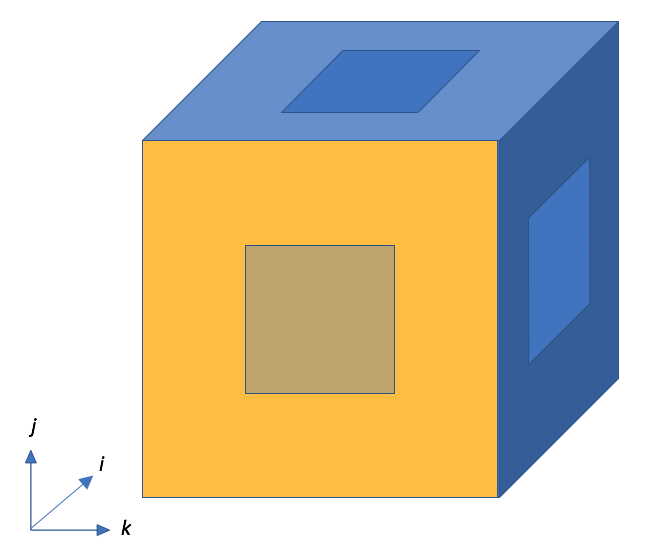
\includegraphics[width = 0.7\textwidth]{../pics/justbox.png}
\end{center}
\caption{\label{justbox} An image indicating the orientation of our cubic satellite in space, alongside the position of the interior cube, marked on the outer faces.}
\end{figure}
\subsection*{Temperature Results}
Because our result data is a temperature at each point in 3D space, we are left with four dimensional results.  Visualization of this is easiest with 3D cross-sectioned images, which are shown below.

If we first look at cross-sections of the temperature with constant $j$ and $k$ in figures \ref{centeredj} and \ref{centeredk}, we see exactly what we would expect on the edges: linear trends on the boundaries.  This is how we initialized our satellite faces through $i$, so this makes sense.  In the center of the box, we have a square with constant temperature 100 K--the aluminum center.  Between these two boundaries, the linear gradient through $i$ persists, interrupted only by a decaying curve between the gradient and the aluminum center's 100 K.

The decaying curve makes sense, since the aluminum center at 100 K is generally cooler than the outside faces, so it acts almost as a heat sink, cooling the immediate area surrounding it.  The linear trend throughout the system is consistent with the steady state solution to the heat equation as well, which is linear. \cite{heateq}

\begin{figure}[h!]
\begin{center}
\begin{subfigure}{0.3\textwidth}
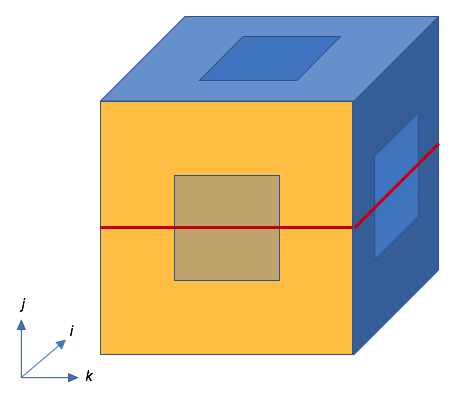
\includegraphics[width=\linewidth]{../pics/centeredjpic.png}
\caption{\label{centeredjpic}}
\end{subfigure}
\begin{subfigure}{0.6\textwidth}
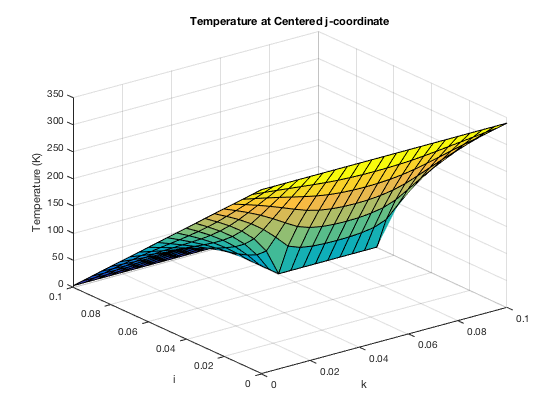
\includegraphics[width=\linewidth]{../pics/centeredj.png}
\caption{\label{centeredj}}
\end{subfigure}
\caption{A plot of temperature through a cross-section at the center of the $j$-axis.  There is a noticeable exponential towards the aluminum center temperature (100 K), however, the trend through $i$ is linear.}
\end{center}
\end{figure}

Our cross section in $k$ shown in fig. \ref{centeredk} is an identical plot to fig. \ref{centeredj}.  This is not a surprise, as the main condition that governs these axes is the linear gradient in $i$ (present in both graphs) and has decaying curves near the internal aluminum box.

\begin{figure}[h!]
\begin{center}
\begin{subfigure}{0.3\textwidth}
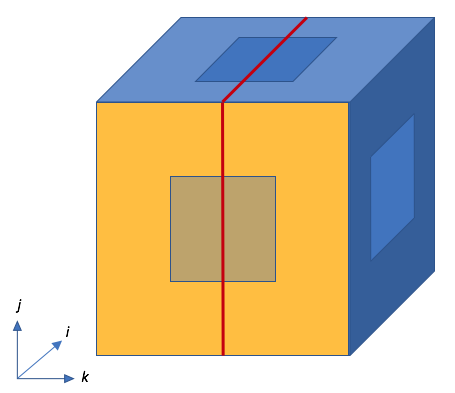
\includegraphics[width=\linewidth]{../pics/centeredkpic.png}
\caption{\label{centeredkpic}}
\end{subfigure}
\begin{subfigure}{0.6\textwidth}
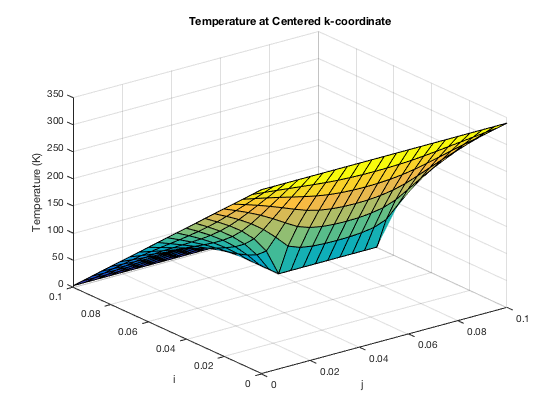
\includegraphics[width=\linewidth]{../pics/centeredk.png}
\caption{\label{centeredk}}
\end{subfigure}
\caption{A plot of temperature through a cross-section at the center of the $k$-axis.  There is a noticeable exponential curve towards the aluminum center temperature (100 K), however, the trend through $i$ is linear.}
\end{center}
\end{figure}

A slightly more interesting image is a cross section as constant $i$, shown in fig. \ref{centeredi}.  The boundaries of the plot all start at the middle of the temperature gradient, then follow our previously shown decay curves to the 100 K aluminum center.  This again makes sense as the satellite center acts as a form of heat sink to the heat absorbed by the sun face.  Each cross section with constant $i$ takes a similar shape to this, with varying depths of the decay curve as the temperature is closer or further from 100 K.

%CENTERED I PIC
\begin{figure}[h!]
\begin{center}
\begin{subfigure}{0.3\textwidth}
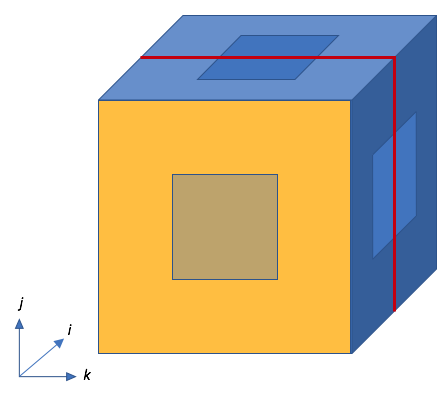
\includegraphics[width=\linewidth]{../pics/centeredipic.png}
\caption{\label{centeredipic}}
\end{subfigure}
\begin{subfigure}{0.6\textwidth}
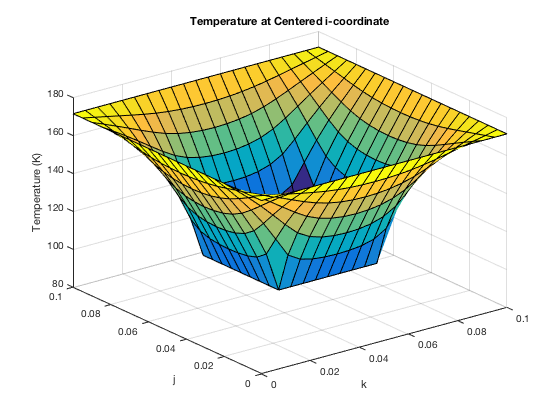
\includegraphics[width=\linewidth]{../pics/centeredi.png}
\caption{\label{centeredi}}
\end{subfigure}
\caption{A plot of temperature through a cross-section at the center of the $i$-axis.  There is a noticeable exponential curve downward from the position in the edge gradient towards the aluminum box center.}
\end{center}
\end{figure}

Overall, the resulting temperature distribution from our system of equations fulfill all expectations from a steady-state system's temperature with two ends held at constant temperatures.  The linear gradient between the temperature of the sun-facing side and the temperature of the cosmic microwave background reaches to the inside of the satellite, only altered by the heat-sink-like presence of the aluminum center, which is generally lower in temperature than most of the box interior.
\subsection*{Computational Results}
Computationally, both methods produce answers that concur up to 12 decimal places ($10^{-13}\%$ maximum difference).  This is due partially to the code written for this assignment using full pivoting.  Full pivoting solves matrix equations while ensuring the largest value in the matrix is always moved to the diagonal by shifting rows and columns.  This results in less opportunities for numerical error.

Despite these definite equivalencies in numerical solutions, there is a massive disparity in the computation time required for each method.  $LAPACK$ is highly optimized for quick computation, and runs at an average of twenty times faster than the basic $LU$ factorization code.  For example, with a $11\times 11\times 11$ mesh in this system, the $LU$ factorization code takes approximately 19.934 seconds to run, compared to the $5.5\times 10^{-5}$ seconds for $LAPACK$, even in double precision accuracy.

Overall, the steady-state behavior of the satellite's temperature behaves as expected: a linear gradient with $i$ away from the sun, and a general temperature decay curve moving inward to the 100 K aluminum center.  In the long-term steady-state solution, the system's various materials make no contribution, and the satellite behaves as if it were simply a uniform material with a 100 K center and sides initialized as described above.  Provided polysilicon adequately serves its structural and electrical purposes at both 340 K and ~2 K, the satellite should be safe in its expected location in space.

The solution to this system using a $LU$ factorization code yields comparable results to those from the highly optimized $LAPACK$ within $10^{-12}\%$.  The runtime between two methods illustrates the definite preference for $LAPACK$ due to its nearly twenty-fold speed advantage.
\newpage
\bibliographystyle{plain}
\bibliography{sources}
\newpage
\section*{Appendix}
Attached is the source code for this project, written in Fortran.
\lstinputlisting[language=Fortran]{../ssheateq.f90}
\subsection*{MATLAB Plotting Script}
\lstinputlisting[language=Octave]{../plots.m}
\end{document}